\section{Shape Matching}
\label{sec:shape-matching}
The shape matching problem is to find a mapping between shapes.
For an illustration see Figure~\ref{fig:shape-matching}.
We follow the shape matching formulation of~\cite{windheuser2011geometrically,windheuser2011large}. Here the shape matching problem is posed as an ILP which ensures an orientation preserving geometrically consistent matching.

\begin{figure}[H]
	\begin{center}
		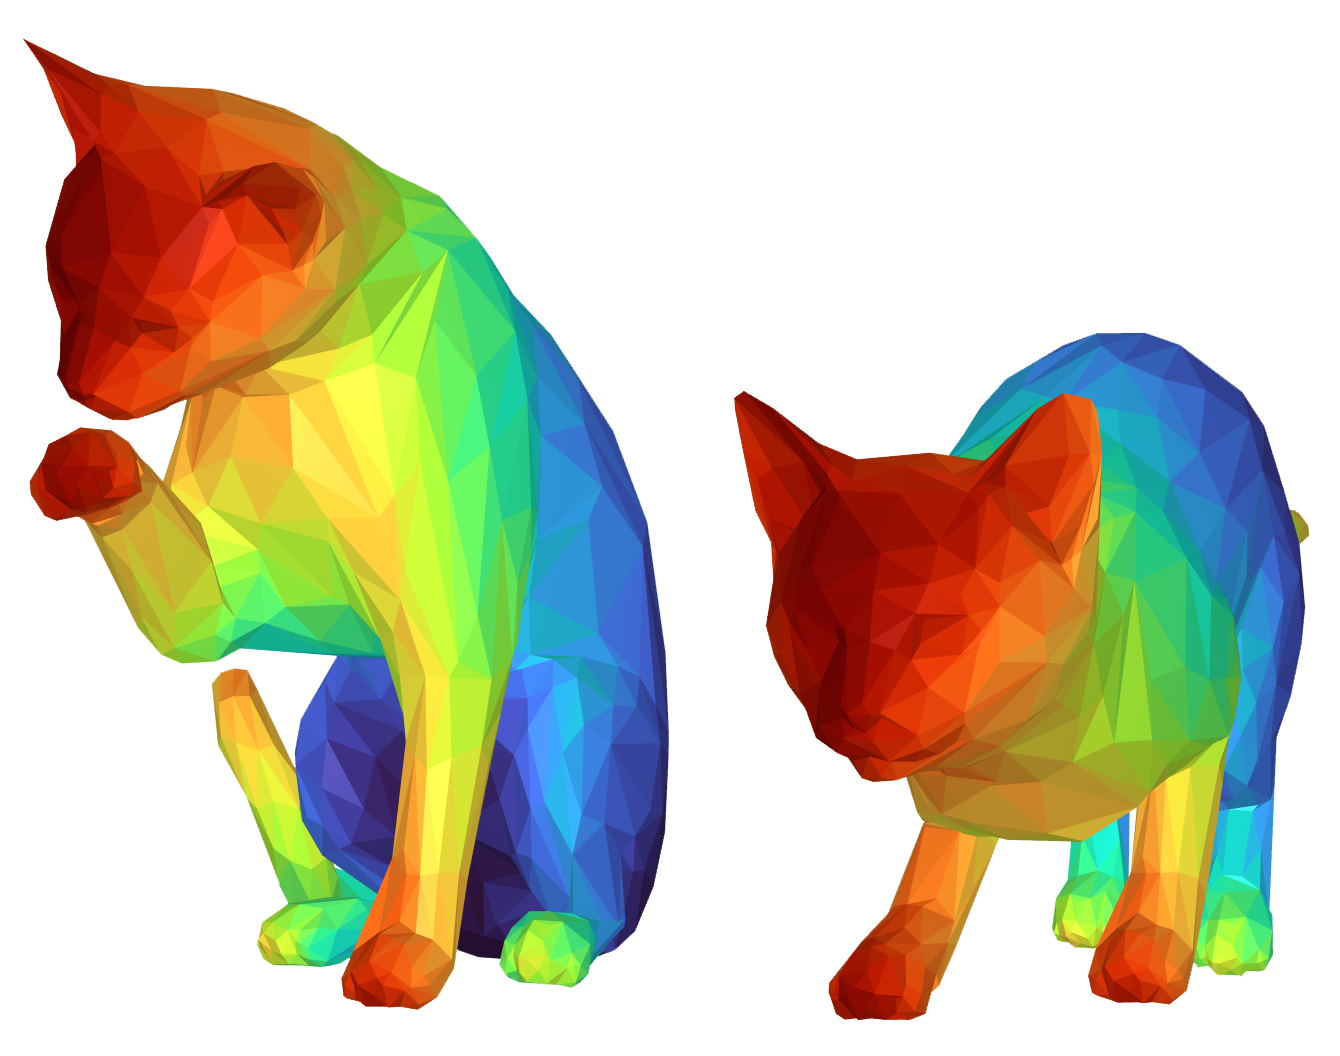
\includegraphics[width=0.8\columnwidth]{images/cat-matching}
	\end{center}
	\caption{Shape matching of a cat in different poses. Colors encode matches of triangles.}
	\label{fig:shape-matching}
\end{figure}

\begin{definition}[Shape]
	We define a shape $X$ as a triplet $(V_X, E_X,F_X)$ of vertices $V_X$, 
	edges 
	$E_X \subset V_X \times V_X$ 
	and triangles 
	$F_X \subset V_X \times V_X \times V_X$,
	such that the manifold induced by the triangles is oriented and has no boundaries.
\end{definition}

\begin{definition}[Degenerate Triangles and Edges]
	By $\overline{F}_\bullet$ we denote the set of \emph{degenerate} triangles, that in addition to the triangles $F_\bullet$ also contains triangles formed by edges (a triangle with two vertices at the same position) and triangles formed by vertices (a triangle with three vertices at the same position).
	Similarly, we consider the set of degenerate edges $\overline{E}_\bullet$.
\end{definition}


\begin{definition}[Product Spaces]
	Let two shapes $X$ and $Y$ be given.
	The triangle product space is defined as
	\begin{equation}
		F \coloneqq \left\{ 
		\begin{pmatrix}
			a_1, b_1 \\
			a_2, b_2 \\ 
			a_3, b_3
		\end{pmatrix} \left|
		\begin{array}{ll}
			(a_1 a_2 a_3 \in F_X \wedge b_1 b_2 b_3 \in \overline{F}_Y )~\vee \\
			(a_1 a_2 a_3 \in \overline{F}_X \wedge b_1 b_2 b_3 \in {F}_Y ) 
		\end{array} \right.
		\right\}.\nonumber
	\end{equation}
	
	The edge product space is defined as
	\begin{equation}
		E \coloneqq \left\{ 
		\begin{pmatrix}
			a_1, b_1 \\
			a_2, b_2
		\end{pmatrix} \left|
		\begin{array}{ll}
			(a_1 a_2 \in E_X \wedge b_1 b_2 \in \overline{E}_Y )~\vee\\
			(a_1 a_2 \in \overline{E}_X \wedge b_1 b_2 \in {E}_Y )
		\end{array} \right.
		\right\}.\nonumber
	\end{equation}
\end{definition}

\begin{definition}[Discrete Surfaces]
	Let the triangle product space $F$ and the edge product space $E$ be given for a pair of shapes $X, Y$. A discrete surface $\Gamma \subset F$  is given by its indicator representation 
	\begin{equation}
		\Gamma = \{0, 1\}^{|F|}.
	\end{equation}
	The $f$-th entry $\Gamma_f$ belongs to the $f$-th triangle product in $F$.
\end{definition}
Triangle products encode a matching between a triangle from $X$ and a triangle from $Y$. Hence, discrete surfaces encode a matching between $X$ and $Y$. Constraints are needed to ensure surjectivity and geometric consistency of the matching. 

\begin{definition}[Projection Operator]
	The projection $\pi_X : F \rightarrow \Z^{\abs{F_X}}$ is defined by
	\begin{equation}
        (\pi_x \Gamma)_{a_1 a_2 a_3} = \sum_{\left\{ f \in F : f = \begin{pmatrix} a_1, b_1\\ a_2, b_2 \\ a_3, b_3 \end{pmatrix}\right\}} \Gamma_f\,.
	\end{equation}
    for all non-degenerate triangles $a_1 a_2 a_3 \in F_X$.

	The projection operator $\pi_Y$ is defined analoguously.
\end{definition}

\begin{definition}[Surjectivity Constraint]
	A given discrete surface $\Gamma$ ensures a surjective matching of $X$ with $Y$ if it projects to each shape $X$ and $Y$ such that
	\begin{equation}
			\begin{pmatrix}
			\pi_X \\ \pi_Y
		\end{pmatrix}
		\Gamma
		= 
		\begin{pmatrix}
			\boldsymbol{1}_{|F_X|} \\ \boldsymbol{1}_{|F_Y|}
		\end{pmatrix},
	\end{equation}
	with $\boldsymbol{1}_{|F_X|} \in \{1\}^{|F_X|}$ and $\boldsymbol{1}_{|F_Y|} \in \{1\}^{|F_Y|}$.
\end{definition}

\begin{definition}[Orientation]
	For the sets $E_X$ and $E_Y$ an arbitrary orientation shall be defined. This implies an orientation for each edge product $e = \begin{pmatrix} a_1,b_1 \\ a_2,b_2 \end{pmatrix} \in E$.
	By means of these orientations a vector $O\begin{pmatrix}e\end{pmatrix} \in \Z^{\abs{E}}$ can be defined for every edge product $e$. The entries of $O\begin{pmatrix}e\end{pmatrix}$ write as
	\begin{equation}
		O(e) = \begin{cases}
			1,& \emph{if } e \in E\\
			-1,& \emph{if } -e \in E\\
			0,& \text{otherwise}
		\end{cases}
	\end{equation}
\end{definition}

\begin{definition}[Boundary Operator]
	The boundary operator $\partial : F \rightarrow \Z^{\abs{E}}$ is defined for every triangle product by
	\begin{equation}
		\partial \begin{pmatrix} a_1, b_1 \\ a_2, b_2 \\ a_3, b_3 \end{pmatrix}
		=
		O\begin{pmatrix} a_1,b_1 \\ a_2,b_2 \end{pmatrix}
		+
		O\begin{pmatrix} a_2,b_2 \\ a_3,b_3 \end{pmatrix}
		+
		O\begin{pmatrix} a_3,b_3 \\ a_1,b_1 \end{pmatrix}
	\end{equation}
	where $a_i$ and $b_i$ form triangles in $X$ resp.\ $Y$ and $\begin{pmatrix} a_i,b_i \\ a_j,b_j \end{pmatrix}$ is the edge product connecting the product vertices $(a_i,b_i)$ and $(a_j,b_j)$.
\end{definition}

\begin{definition}[Closeness/Geometric Consistency Constraint]
	A given discrete surface $\Gamma$ ensures a geometric consistent matching of $X$ with $Y$, i.e. is a closed discrete surface if it satisfies
	\begin{equation}
		\partial
		\Gamma
		= 
		\boldsymbol{0}_{|E|}.
	\end{equation}
\end{definition}

\begin{definition}[Discrete Graph Surfaces]
	A graph surface is a discrete surface which fulfills the geometric consistency constraint as well as the surjectivity constraints.
\end{definition}

\begin{definition}[Deformation Energy]
	The deformation energy $ \mathbb{E}$ is defined for every triangle product. It describes the energy needed to deform the respective triangle from shape $X$ into the triangle from shape $Y$ and vice versa.
\end{definition}

We now have all operators to define the shape matching problem as the search for a discrete graph surface.
\begin{definition}[Shape Matching]
	Given an energy $\mathbb{E} \in \R^{\abs{F}}$ the shape matching problem is
	\begin{equation} 
		\underset{\Gamma \in \{0, 1\}^{|F|}}{\min} \mathbb{E}^\top  \Gamma  
		~~  \text{s.t.} ~~
		\begin{pmatrix}
			\pi_X \\ \pi_Y \\ \partial
		\end{pmatrix}
		\Gamma
		= 
		\begin{pmatrix}
			\boldsymbol{1}_{|F_X|} \\ \boldsymbol{1}_{|F_Y|} \\ \boldsymbol{0}_{\abs{E}} \\
		\end{pmatrix},
		\label{eq:shape-matching-opt}
	\end{equation}
\end{definition}

\subsection{File Format}
Instances are given in the ILP file format from Section~\ref{sec:ilp-file-format}. The filenames contain information about the respective problems
\begin{equation}
	\begin{aligned}
	&\texttt{<\# binvars>\_<\# constraints>\_<shape X>\_} \\
	&\texttt{<\# triangles>\_<shape Y>\_<\#  triangles>.lp}
	\end{aligned}
\end{equation}
Each binary variable belongs to a triangle product. Considering a vertices of shape $X$ as $a_i$ and a vertices of shape $Y$ as $b_i$ respectively. The names of the binary variables are structured as follows 
\begin{equation}
	\texttt{x} \_ \texttt{a}_1 \_ \texttt{a}_2 \_ \texttt{a}_3 \_\_ \texttt{b}_1 \_ \texttt{b}_2 \_ \texttt{b}_3.
\end{equation}
From the names the respective vertices or rather the respective triangle products can be identified.


\subsection{Datasets}
\subsubsection[TOSCA]{TOSCA~\footnote{\url{https://keeper.mpdl.mpg.de/f/cf736ce0e16d4323a13b/?dl=1}}}
A sample generated matching problems (LP-files) on TOSCA~\cite{bronstein2008} shapes. 
The dataset contains $75$ ILP files consisting of problems with $200,000$ binary variables up to $5,000,00$ binary variables.
The dataset contains matching problems between complete shapes and partial shapes and shapes with equal triangulation. Partial shapes are shapes which are missing parts of the original shape (such files are denoted with \texttt{\_partial}). Additionally, there are matching problems which are between non-isometric deformed shapes e.g. a cat matched with a dog (such files are denoted with \texttt{\_noniso}).
\\
The original shapes are not included.

\subsection{Algorithms}
\begin{description}	
	\item[LP + incremental fixation~\cite{windheuser2011geometrically}:]
	LP relaxation of~\eqref{eq:shape-matching-opt} is solved with CPLEX~\cite{cplex} and franctional variables are incrementally fixed towards $\{0,1\}$-values they are close to.
	\item[Eckstein-Bertsekas~\cite{windheuser2011large}:]
	A GPU implementation of the parallelizable primal-dual algorithm proposed by Eckstein and Bertsekas~\cite{eckstein1990alternating}.
\end{description}
